% The Why of Tali Forth
% Scot W. Stevenson

\section{The big picture}

This section provides background information on Forth, the 6502 processor, and
what anybody would want to combine the two. It can be safely skipped.

\subsection{The 6502 MPU}

Humanity reached the high point of processor design with the 6502 in 1976.
Designed by a team including Chuck Peddle and Bill Mensch, it was the engine
that powered the 8-bit home computer revolution of the 1980s.\footnote{Rumor has
it that there was another MPU called `Z80', at the same time, but it ended up
being a footnote.} The VIC-20, Commodore PET, Apple II, and Atari 800 all used
the 6502, among others. 

\begin{figure}[h !]
        \centering
        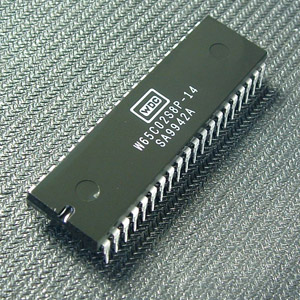
\includegraphics[width=0.5\textwidth]{pics/W65c02}
        \caption{\textit{The 65c02 MPU.} Photographer: Anthony King, released in 
        the public domain}
        \label{fig:65c02}
\end{figure}

More than 40 years later, the processor is still in production by the \href
{http://www.westerndesigncenter.com/wdc/w65c02s-chip.cfm} {Western Design
Center}. Apart for commercial uses, there is an active hobbyist scene centered
on the website \href {http://6502.org/}{6502.org}. Quite a number of people
have built their own 8-bit computers based on this chip. 

The variant produced today is the \href
{https://en.wikipedia.org/wiki/WDC\_65C02}{65c02}, a CMOS chip with some
additional instructions. Tali Forth 2 is specifically designed for this chip and
this chip only.


\subsection{Forth}

Forth 


\section{On writing your own Forth}
